%
% CAPITULO MODELO Y EL EFECTO DE UNA REPULSION coulombiANA
%
\chapter{Modelo incluyendo el efecto de una repulsi\'{o}n coulombiana $V$}
En contraste con el modelo de Ricco et alia, nosotros consideramos un hamiltoniano que no ignore estados de m\'{a}s alta energ\'{i}a. El porqu\'{e} de esta decisi\'{o}n se discutir\'{a} m\'{a}s adelante pero crudamente se puede decir que estos estados de alta energ\'{i}a son escenciales para mantener la robustez de los MZMs. El modelo que se propone en la tesis es el de un nanocable unidimensional en el r\'{e}gimen de electrones sin esp\'{i}n acoplado en su de su extremo izquierdo con un punto cu\'{a}ntico. Existir\'{a} una probabilidad de salto entre el punto cu\'{a}ntico y el sitio m\'{a}s cercano a este en la cadena y un t\'{e}rmino de repulsi\'{o}n coulombiana entre los electrones de ambos sitios. 
\begin{eqnarray}
H &=&\sum_{j=1}^{N-1}(-tc_{j+1}^{\dagger }c_{j}+\Delta c_{j+1}^{\dagger
}c_{j}^{\dagger }+\mathrm{H.c.})-\mu \sum_{j=1}^{N}c_{j}^{\dagger }c_{j} 
\notag \\
&&+\epsilon_{d}d^{\dagger }d-t^\prime (d^{\dagger }c_{1}+\mathrm{H.c.}) \notag \\
&&+V\left( n_d  -\frac{1}{2} \right) 
\left( n_1 -\frac{1}{2} \right),  \label{ham}
\end{eqnarray}
Los primeros dos t\'{e}rminos del hamiltoniano describen a la cadena de Kitaev donde $t$ es el hopping entre sitios, $\Delta$ el gap superconductor, y $\mu$ es potencial qu\'{i}mico de la cadena. Los dos t\'{e}rminos que siguen describen la energ\'{i}a del punto cu\'{a}ntico y el hopping entre el punto y el primer sitio de la cadena. Finalmente, El \'{u}ltimo t\'{e}rmino describe la repulsi\'{o}n coulombiana entre el punto cu\'{a}ntico y el primer sitio de la cadena.

Escogemos tratar el t\'{e}rmino de repulsi\'{o}n coulombiana en la aproximaci\'{o}n Hartree-Fock no restringida. Adem\'{a}s de ser un enfoque razonable para tratar con el sistema, nos permite ciertas facilidades computacionales.

La estrategia es aplicar el mapeo de la secci\'{o}n 1.3  pero a nuestro hamiltoniano. Se aplic\'{o} el mapeo ya en la cadena de Kitaev en (\ref{kitaev_matrix_element}) así que queda hacer el mapeo de términos que incluyan operadores del punto cuántico. Nos concentramos en el término de interacción $V(n_d-\frac{1}{2})(n_1-\frac{1}{2})$. En su forma de Hartree-Fock irrestricto luce como 
\begin{eqnarray}
n_{d}n_{1} &\simeq &\left\langle n_{d}\right\rangle n_{1}+n_{d}\left\langle
n_{1}\right\rangle -\left\langle n_{d}\right\rangle \left\langle
n_{1}\right\rangle   \notag \\
&&-\left\langle d^{\dagger }c_{1}\right\rangle c_{1}^{\dagger }d-d^{\dagger
}c_{1}\left\langle c_{1}^{\dagger }d\right\rangle +\left\langle d^{\dagger
}c_{1}\right\rangle \left\langle c_{1}^{\dagger }d\right\rangle   \notag \\
&&+\left\langle d^{\dagger }c_{1}^{\dagger }\right\rangle c_{1}d+d^{\dagger
}c_{1}^{\dagger }\left\langle c_{1}d\right\rangle -\left\langle d^{\dagger
}c_{1}^{\dagger }\right\rangle \left\langle c_{1}d\right\rangle .  \label{hf}
\end{eqnarray}
\par Para derivar los elementos de matriz del hamiltoniano iremos por partes, primero tratanto la cadena sola, y luego cada t\'{e}rmino del desacople por separado para saber de d\'{o}nde viene cada parte. Los elementos de matriz de la cadena ya pueden ser calculados a partir de la ecuaci\'{o}n (\ref{kitaev_matrix_element}). Entonces lo que queda calcular son los elementos de matriz que tengan que ver con el punto cu\'{a}ntico, es decir, el n\'{u}mero de ocupaci\'{o}n del punto, t\'{e}rmino de hopping y el t\'{e}rmino de repulsi\'{o}n.  
\begin{equation}
    \begin{matrix}
    \bra{d,c}\tilde H\ket{d,c}= \epsilon_d + V\langle n_1\rangle & \bra{d,a}\tilde H\ket{d,a}= -\epsilon_d - V\langle n_1\rangle\\
     \bra{1,c}\tilde H\ket{d,c} = -t' - V\langle c^\dagger_d c_1\rangle & \bra{1,a}\tilde H\ket{d,a} = t' + V\langle c^\dagger_d c_1\rangle\\
      \bra{d,c}\tilde H\ket{1,a} = -V\langle c^\dagger_d c^\dagger_1 \rangle & \bra{d,a}\tilde H\ket{1,c} = V\langle c^\dagger_d c^\dagger_1 \rangle\\
      \bra{1,c}\tilde H\ket{1,c} = ...+ V\langle n_d\rangle & \bra{1,a}\tilde H\ket{1,a} = ...- V\langle n_d\rangle
    \end{matrix}
\end{equation}
Una vez que ya sabemos las dependencias de los elementos de matriz debemos diagonalizar $\tilde H$ y hallar los valores de expectaci\'{o}n de forma autoconsistente. Esto se calcula en la siguiente subsecci\'{o}n.
\par Muchas de las referencias trabajan cambiando no el potencial qu\'{i}mico pero s\'{i} la energ\'{i}a de ocupaci\'{o}n del punto cu\'{a}ntico (que experimentalmente se puede cambiar con un potencial de compuerta) lo que se adopta tambi\'{e}n en esta tesis. Sacamos los perfiles de baja energ\'{i}a cambiando los valores de $\epsilon_d$. Estos se explicar\'{a}n m\'{a}s a fondo en la siguientes secciones haciendo una comparaci\'{o}n con el paper de Ricco \emph{et alia}, pero a grandes razgos en la figura \ref{comparacion1} donde se pueden apreciar los MZMs que son aquellos estados que se encuentran cercanos a una energ\'{i}a cero, y el efecto que tiene el punto cu\'{a}ntico en los estados de m\'{a}s alta energ\'{i}a en la cadena en, particular que ocurre cerca a $\epsilon_d=0$. 
% VALORES DE EXPECTACION Y CALCULOS
%
\section{Valores de expectaci\'{o}n y c\'{a}lculos}
Ya que buscamos diagonalizar el hamiltoniano, lo que en escencia necesitamos calcular son los estados $\gamma_\nu$ tal que $[H,\gamma^\dagger_\nu]=E_\nu\gamma_\nu^\dagger$. Si recordamos las ecuaciones \ref{mapeo1} y \ref{mapeo2}, lo que esto nos quiere decir en t\'{e}rminos de kets es que $\ket{\gamma,c}$ ser\'{a} uno de los autoestados de $\tilde H$.
Usando el enfoque de BCS haremos un cambio de base y pasaremos de operadores $c_i$ a $\gamma_\nu$ donde existe una forma de definir $c$ en terminos de $\gamma$ y viceversa
\begin{equation}
\begin{split}
        c_i^\dagger&=\sum_{\nu'}\Big( \overline{D}_{i\nu'}\gamma^\dagger_{\nu'}+\overline{E}_{i\nu'}\gamma_{\nu'} \Big)\\
        c_i&=\sum_{\nu'}\Big( D_{i\nu'}\gamma_{\nu'}+E_{i\nu'}\gamma^\dagger_{\nu'} \Big).
\end{split}
\label{eq:c_to_gamma}
\end{equation}
As\'{i}mismo los $\gamma_\nu$ en general tendr\'{a}n la forma: 
\begin{equation}
    \begin{split}
         \gamma^\dagger_\nu&=\sum_{i}\Big( \overline{A}_{i\nu}c^\dagger_{i}+\overline{B}_{i\nu}c_{i} \Big)\\
        \gamma_\nu&=\sum_{i}\Big( A_{i\nu}c_{i}+B_{i\nu'}c^\dagger_{i} \Big).       
    \end{split}
    \label{eq:gamma_to_c}
\end{equation}
Para relacionar $\gamma_\nu$ y $c_i$ a trav\'{e}s de las matrices $A$, $B$, $C$, y $D$, calculamos sus relaciones de conmutaci\'{o}n primero dejando el segundo operador fijo, mientras que el otro lo expresamos usando las ecuaciones de arriba.
\begin{equation}
    \{\gamma^\dagger_\nu,c_j\}=\Big\{\sum_i \overline{A}_{\nu i} c_i^\dagger+\overline{B}_{\nu i}c_i,c_j\Big\}=\Big\{\sum_i \overline{A}_{\nu i} c_i^\dagger,c_j\Big\}=\overline{A}_{\nu j},
\end{equation}
ahora si dejo fijo el operador de $\gamma_\nu$
\begin{equation}
    \{\gamma^\dagger_\nu,c_j\}=\Big\{\sum_i D_{i \nu} \gamma_\nu+E_{i \nu}\gamma^\dagger_\nu\Big\}=\Big\{\gamma^\dagger_\nu,\sum_i D_{i \nu} \gamma_i^\dagger\Big\}=D_{i \nu}.
\end{equation}
Si realizamos el mismo c\'{a}lculo para el anticonmutador $\{\gamma_\nu,c_i\}$ se obtiene que $E_{i\nu}=B_{\nu i}$. 
\begin{equation}
    \overline{A}=D,\quad E=B
    \label{rela_mat}
\end{equation}
Una vez diagonalizado computacionalmente $\tilde H$, conocemos $A$ y $ B$, por lo tanto por la ecuaci\'{o}n (\ref{rela_mat}) llegamos a saber tambi\'{e}n los valores de $E_{i\nu}$ como $D_{i\nu}$. Como ya hemos mencionado, los operadores $\gamma^\dagger_\nu$ y $\gamma_\nu$ se identifican como a los autoestados de $\tilde H$, donde $\gamma^\dagger_\nu$ corresponde a los a los autoestados con energ\'{i}a $E_\nu$ positiva y $\gamma_\nu$ con los de energ\'{i}a negativa. Esto se puede derivar del m\'{e}todo de mapeo expuesto y que $[H,\gamma_\nu^\dagger]=E_\nu \gamma^\dagger_\nu \Rightarrow [H,\gamma_\nu]=-E_\nu \gamma_\nu$.\\
Como ejemplo del c\'{a}lculo del valor de expectaci\'{o}n tomamos $\langle c^\dagger_j c_i \rangle$. Al conocer la expresi\'{o}n de $c^\dagger_i$ y$c_i$ en t\'{e}rminos de los $\gamma_\nu$ y $\gamma_\nu^\dagger$, y las matrices $D_{i\nu}$ y $E_{i\nu}$ luego de la diagonalizaci\'{o}n, queda reemplazar (\ref{eq:c_to_gamma}) y evaluarlos en su estado fundamental correspondiente. Cabe recordar que el estado fundamental en el espacio de operadores $\gamma_\nu$ est\'{a} dado por
\begin{equation}
    \ket{g}=\prod \gamma_\nu \ket0
\end{equation}
%
%
%
\begin{figure}[H]
\begin{center}
\includegraphics*[width=0.7\columnwidth]{ch2f/nd.pdf}\\
\vspace{-1cm}
\includegraphics*[width=0.7\columnwidth]{ch2f/n1.pdf}\\
\vspace{-1cm}
\includegraphics*[width=0.7\columnwidth]{ch2f/c+d.pdf}\\
\vspace{-1cm}
\includegraphics*[width=0.73\columnwidth]{ch2f/cd.pdf}
\end{center}
\caption{Valores de expectaci\'{o}n. (a) Ocupaci\'{o}n del punto cu\'{a}ntico. (b) Ocupaci\'{o}n del primer sitio de la cadena de Kitaev. (c) Salto entre el punto cu\'{a}ntico y el primer sitio de la cadena de Kitaev. (d) Par de Cooper con fermiones del sitio $d$ y el sitio $1$ }
\label{exp_val}
\end{figure}
Calculamos $\langle c_j^\dagger c_i \rangle$:
\begin{equation}
\begin{split}
             \langle c_j^\dagger c_i \rangle &= \bra{g}\Big( \sum_{\nu'}\Big( \overline{D}_{i\nu'}\gamma^\dagger_{\nu'}+\overline{E}_{i\nu'}\gamma_{\nu'} \Big) \Big)\Big( \sum_{\nu'}\Big( D_{i\nu'}\gamma_{\nu'}+E_{i\nu'}\gamma^\dagger_{\nu'} \Big) \Big) \ket{g}\\
             &= \bra{0}_\gamma\sum_{\nu\nu'} \overline{D}_{i\nu'} D_{i\nu} \gamma_{\nu'}^\dagger\gamma_\nu + \overline{D}_{i\nu'}E_{i\nu}\gamma^\dagger_{\nu'}\gamma^\dagger_\nu + \overline{E}_{i\nu'}D_{i\nu}\gamma_{\nu'}\gamma_\nu+\overline{E}_{i\nu'}E_{i\nu} \gamma_{\nu'}\gamma^\dagger_\nu \ket{0}_\gamma\\
             &=\sum_{\nu\nu'} \bra{0}_\gamma \overline{E}_{i\nu'} E_{i\nu} \gamma_{\nu'}\gamma^\dagger_\nu\ket{0}_\gamma \\
             &=\sum_\nu \overline{E}_{j\nu} E_{i\nu}
\end{split}
\end{equation}
Asimismo calculamos los otros valores de expectaci\'{o}n necesarios para completar valores en el hamiltoniano una vez el m\'{e}todo Hartree-Fock es aplicado.
\begin{equation}
    \langle c_j^\dagger c_i \rangle = \sum_\nu \overline{E}_{j\nu} E_{i\nu}, \quad \langle c_j^\dagger c_i^\dagger\rangle = \sum_\nu 
 \overline{E}_{j\nu} \overline{D}_{i\nu}
\end{equation}
Los dem\'{a}s valores de expectaci\'{o}n salen de la relaci\'{o}n $\langle AB\rangle= \overline{\langle B^\dagger a^\dagger \rangle}$. En la figura \ref{exp_val} se presentan los valores de expectaci\'{o}n como funci\'{o}n de la energ\'{i}a de ocupaci\'{o}n del punto cu\'{a}ntico. En la figura \ref{exp_val}(a), cuando $\epsilon_d<0$, se observa que la ocupaci\'{o}n del punto cu\'{a}ntico es $>0.5$ y para $\epsilon_d$ m\'{a}s grande en magnitud que $t'$, $|\epsilon_d|\gg t'$, se nota una ocupaci\'{o}n cerca de $1$. Si hemos de encontrar un electr\'{o}n en el punto cu\'{a}ntico este impone una repulsi\'{o}n coulombiana en sitio adyacente a este, o sea en el sitio $1$. Esta correlaci\'{o}n se hace notar en la figura \ref{exp_val}(b) ya que para $\epsilon_d<0$ el valor de expectacion de la ocupaci\'{o}n del primer sitio de la cadena $\langle c^\dagger_1 c_1 \rangle<0.5$. 

Para entender c\'{o}mo cambian los valores de expectaci\'{o}n del hopping $\langle c_d^\dagger c_1\rangle$ en la figura \ref{exp_val} es \'{u}til pensar en el modelo de la mol\'{e}cula di\'{a}tomica heteronuclear con un solo orbital. En nuestro contexto, uno de los \'{a}tomos corresponde al punto cu\'{a}ntico y el otro al primer sitio de la cadena. Este modelo tiene un hamiltoniano de la forma 
\begin{equation}
    H=\epsilon_d d^\dagger d + \epsilon_c c^\dagger c-t'( d^\dagger c + c^\dagger d).
    \label{hammy_diatomica}
\end{equation}
donde el operador $d$ corresponde al punto cu\'{a}ntico y $c$ al sitio del extremo izquierdo de la cadena.  
Su estado fundamental luce como $\ket{g}=(\alpha d^\dagger+\beta c^\dagger)\ket{0}$, donde se debe cumplir la normalizaci\'{o}n $|\alpha|^2+|\beta|^2=1$.\\
Si, por ejemplo, calculamos el valor de expectaci\'{o}n para el hopping de electrones entre las mol\'{e}culas tendremos
\begin{equation}
    \begin{split}
        \bra{g}c^\dagger d\ket{g}&=\bra{0}(\alpha d+ \beta c)(c^\dagger d)(\alpha d^\dagger + \beta c^\dagger)\ket{0}\\
        &=\bra{0}\beta\alpha\ket0\\
        &=\beta\alpha
    \end{split}
\end{equation}
De la misma manera calculamos
\begin{equation}
  \langle d^\dagger d\rangle=\alpha^2,\quad \langle c^\dagger c\rangle=\beta^2,\quad \langle c^\dagger d \rangle= \beta\alpha
  \label{diato}
\end{equation}
Para comprobar que este modelo sigue de forma qualitativa el mismo comportamiento que los valores de expectaci\'{o}n de la figura \ref{exp_val}, tomamos como un valor de prueba $\alpha^2=0.5$ que corresponde al valor de expectaci\'{o}n de la ocupaci\'{o}n del punto cu\'{a}ntico cuando $\epsilon_d=0$. Incluyendo este valor en los valores de expectaci\'{o}n del modelo de la mol\'{e}cula diat\'{o}mica obtenemos:
\begin{equation}
    \langle d^\dagger d\rangle=0.5,\quad \langle c^\dagger c\rangle=0.5,\quad \langle c^\dagger d\rangle=0.38
\end{equation}
Estos valores van de acuerdo con los valores de expectaci\'{i}n de la figura \ref{exp_val} para el modelo de punto cu\'{a}ntico acoplado a la cadena cuando $\epsilon_d=0$. Se espera que las ecuaciones (\ref{diato}) correspondan de forma aproximada a los valores de expectaci\'{o}n del modelo de la tesis (\ref{ham}) para cualquier valor de $\alpha$ en el rango de valores que toma el valor de expectaci\'{o}n $\langle c_d^\dagger c_d\rangle$ en la figura \ref{exp_val}.
%
%
%
\section{Discusión de la hipótesis de Ricco \emph{et  alia}}
Recordemos que Ricco \emph{et alia} presentan un t\'{e}rmino de repulsi\'{o}n de la forma
\begin{equation}
    Un_d n_f=\frac{1}{2}U n_d\Big( i\gamma_R\gamma_L+\frac{1}{2}\Big).
\end{equation}
Afirman que el modelo que usan es uno efectivo a bajas energ\'{i}as. Es decir, en principio el t\'{e}rmino de repulsi\'{o}n considerando todo el rango de energ\'{i}as es uno donde el acople es con toda la cadena
\begin{equation}
    Un_dn_\omega=Un_d\Big(\sum_i c^\dagger_i c_i\Big)
    \label{eq:repu_comp}
\end{equation}
donde $n_\omega$ significa el n\'{u}mero de ocupaci\'{o}n del cable (\emph{wire}). Queremos indagar qu\'{e} exactamente est\'{a}n dejando de lado y c\'{o}mo eso puede afectar al espectro de energ\'{i}as y a la hibridizaci\'{o}n de los MZMs. 
Vimos en las ecuaciones (\ref{eq:gamma_to_c}) y (\ref{eq:c_to_gamma}) que cuando diagonalizamos $\tilde H$ obtenemos las expresiones de los estados $\gamma^\dagger_\nu$ en relaci\'{o}n a los operadores originales $c^\dagger_i$ y $c_i$. Reemplazamos estos en la expresi\'{o}n de repulsi\'{o}n coulombiana de Ricco \emph{et alia} \ref{eq:repu_comp}. Trabajamos solo $n_\omega$:
\begin{equation}
    \begin{split}
        \sum_i c_i^\dagger c_j&=\sum_i\Big[ 
\sum_{\nu'}(\overline{D}_{i\nu'}\gamma_{\nu'}^\dagger + \overline{E}_{i\nu'}\gamma_{\nu'}) \Big]\Big[ 
\sum_{\nu''}(D_{i\nu''}\gamma_{\nu''} + E_{i\nu''}\gamma^\dagger_{\nu''}) \Big]\\
&=\sum_{i\nu'\nu''}\Big[ \overline{D}_{i\nu'}D_{i\nu''}\gamma_{\nu'}^\dagger\gamma_{\nu''}+\overline{D}_{i\nu'}E_{i\nu''}\gamma^\dagger_{\nu'}\gamma^\dagger_{\nu''}\\
&+\overline{E}_{i\nu'}D_{i\nu''}\gamma_{\nu'}\gamma_{\nu''}+\overline{E}_{i\nu'}E_{i\nu''}\gamma_{\nu'}\gamma^\dagger_{\nu''}\Big]
    \end{split}
\end{equation}
Ahora digamos que $f^\dagger$ es el operador entre los $\gamma_\nu^\dagger$ correspondiente al estado con m\'{a}s baja energ\'{i}a positiva. Sabemos que habr\'{a} uno solo de estos porque estamos en el contexto de un sistema de la cadena de Kitaev en su fase topol\'{o}gica. Luego, el n\'{u}mero de ocupaci\'{o}n lo separamos entre t\'{e}rminos que son acompa\~{n}ados por $f^\dagger$ o $f$ y el resto de estados que sabemos que son de energ\'{i}as mayores.
\begin{equation}
    \begin{split}
        &=\sum_i \overline{D}_{i\nu_f} D_{i\nu_f} f^\dagger f + \overline{E}_{i\nu_f} E_{i\nu_f} f f^\dagger\\
        &+\sum_i\sum_\nu\Big[ \overline{D}_{i\nu_f}D_{i\nu_f} f^\dagger\gamma_\nu + \overline{D}_{i\nu_f} E_{i\nu_f} f^\dagger \gamma_\nu^\dagger\\
        &+\overline{E}_{i\nu_f} D_{i\nu_f} f\gamma_\nu + \overline{E}_{i\nu_f}E_{i\nu_f} f\gamma_\nu^\dagger \Big]\\
        &+...
    \end{split}
\end{equation}
Como estamos interesados estrictamente en bajas energ\'{i}as nos quedamos con los t\'{e}rminos parecidos a $f^\dagger f$ y $ff^\dagger$
\begin{equation}
\begin{split}
    \sim &\sum_i |D_{i\nu_f}|^2f^\dagger f+|E_{i\nu_f}|^2 f f^\dagger\\
    &\sum_i(|D_{i\nu_f}|^2-|E_{i\nu_f}|^2) f^\dagger f + |E_{i\nu_f}|^2
\end{split}
\end{equation}
Una vez que tomamos las energ\'{i}as m\'{a}s bajas el operador de n\'{u}mero queda como 
\begin{equation}
    \sum_i c^\dagger_i c_i \rightarrow \delta f^\dagger f + \tex{cte}
\end{equation}
donde $f$ es el estado de m\'{a}s baja energ\'{i}a formado por los Majorana de los extremos de la cadena $f^\dagger = \gamma_L+i\gamma_R$. Reemplazando esto en el t\'{e}rmino de interacci\'{o}n de la ecuaci\'{o}n (\ref{eq:repu_comp}) llegamos a lo propuesto por Ricco \emph{et alia}, pero con un $\delta$ en general bastante menor a $1$.

Por otro lado, ir a trav\'{e}s de los detalles de las simplificaciones que tomaron nos deja entrever que quiz\'{a}s tomar un enfoque de hamiltoniano efectivo no es lo m\'{a}s apropiado ya que dejar de lado estados de m\'{a}s energ\'{i}a significar\'{i}a evitar ciertas mezclas entre estados que podr\'{i}an compensar la separaci\'{o}n extra que implica $n_dn_f$. De hacer un campo medio restringido a este t\'{e}rmino nos da
\begin{equation}
    \langle n_d \rangle n_f+\langle n_f \rangle n_d -\langle n_d\rangle \langle n_f\rangle
\end{equation}
donde observamos que $n_f\langle n_d\rangle$ contribuye al t\'{e}rmino $\epsilon_M\gamma_L\gamma_R$ en (\ref{hammy_ricco}). Podr\'{i}amos pensar en la cadena aislada de Kitaev donde incluso moviendo el potencial qu\'{i}mico seguiremos observando MZMs porque estos se reacomodan al nuevo $\mu$. Son distintos en forma a los MZMs anteriores pero a\'{u}n presentan una energ\'{i}a cercana a cero. 

En esta tesis presentamos un modelo m\'{a}s realista. Modelamos la repulsi\'{o}n como 
\begin{equation}
    H_V=n_d n_1
\end{equation}
el cual tratamos en la aproximaci\'{o}n de Hartree-Fock irrestricto. Esta forma de modelar la difiere de la de Ricco \emph{et alia} y suponemos que es m\'{a}s realista. Pensamos que es razonable que el papel que juega el Majorana del extremo derecho no ser\'{a} muy importante ya que a m\'{a}s distancia menor es la repulsi\'{o}n coulombiana. Adem\'{a}s, para tomar en cuenta estados de m\'{a}s alta energ\'{i}a, incluimos toda la cadena de Kitaev. Asimismo, permitimos que haya una probabilidad de salto $t'$ de electrones entre el punto cu\'{a}ntico y el primer sitio.
%
% COMPARACION DE RESULTADOS CON EL NUVO MODELO
%
\section{Comparaci\'{o}n de resultados con el nuevo modelo} Los resultados que se presentan en esta secci\'{o}n refuerzan y extienden lo ya mencionado en la secci\'{o}n de anterior ya que a trav\'{e}s de simulaciones del espectro de energ\'{i}a del sistema y variando el par\'{a}metro de la energ\'{i}a de ocupaci\'{o}n del punto cu\'{a}ntico $\epsilon_d$ se observa que en realidad los modos cero de Majorana son robustos ante la presencia de la repulsi\'{o}n coulombiana.

En la figura \ref{comparacion1}, se muestra el espectro de bajas energ\'{i}as del modelo usado en la tesis para el caso de una cadena de $N=20$ sitios, $\mu=0$, $\Delta=0.2$, $t=1$ y $t'=0.2$. Estos perfiles est\'{a}n dados con respecto a c\'{o}mo va cambiando el nivel de energ\'{i}a del punto cu\'{a}ntico. Para estudiar c\'{o}mo el t\'{e}rmino de repulsion interat\'{o}mica afecta al sistema analizamos los casos en los que $V=0$ y $V=1$. Para el caso de $V=0$ vemos que los MZMs poseen una forma de mo\~{n}o y existe una brecha de energ\'{i}a relevante entre ellos y estados de m\'{a}s alta energ\'{i}a. El sistema tambi\'{e}n fue analizado en una cadena de $N=50$ sitios pero por conveniencia para apreciar m\'{a}s los MZMs nos quedaremos con el caso de $20$ (por ahora) ya que sabemos que la separaci\'{o}n de los MZMs decae exponencialmente con la longitud de la cadena. Ahora bien, al prender el t\'{e}rmino de repulsion coulombiana, $V=1$, y si uno siguiera el trabajo de Ricco et alia uno esperar\'{i}a observar un separaci\'{o}n mayor en las energ\'{i}as de los MZMs, pero lo que se ve en la figura \ref{comparacion1} cuando $V=1$ es que los MZMs siguen ah\'{i} y, en todo caso, la separaci\'{o}n se hace menor. Es decir, no solo son robustos ante la perturbaci\'{o}n que $V$ impone en el sistema, sino que cuando la repulsi\'{o}n est\'{a} presente los vuelve m\'{a}s robustos.\\

En la figura \ref{comparacion1}, tambi\'{e}n notamos que para valores cercanos a $\epsilon_d=0$ existe una deformaci\'{o}n en la forma del espectro de energ\'{i}as. Si recordamos el espectro de energ\'{i}as para una cadena de Kitaev aislada para $\mu=0$ en la figura \ref{fig:kitaev}, notamos que hay dos energ\'{i}as sim\'{e}tricas $\sim 0.4$ y $\sim -0.4$ para una cadena de $N=20$ sitios. Estas corresponder\'{i}an (aproximadamente) a las que observamos para un $|\epsilon_d|\geq 0.5$ en la figura \ref{comparacion1}. Para $|\epsilon_d|\leq 0.5$ nos preguntamos qu\'{e} est\'{a} causando la deformaci\'{o}n y una explicaci\'{o}n es dada por el modelo de la mol\'{e}cula diat\'{o}mica heteronuclear que, recordemos, trata de modelar lo que pasa solo entre el punto cu\'{a}ntico y el primer sitio de la cadena. Tomamos de nuevo el hamiltoniano (\ref{hammy_diatomica}) con $\epsilon_c=0$ y computamos su espectro de energ\'{i}as en funci\'{o}n de $\epsilon_d$ las autoenerg\'{i}as con
\begin{equation}
    E_m=\frac{1}{2}[(\epsilon_d+\epsilon_c)\pm \sqrt{(\epsilon_d-\epsilon_c)^2+4t^2}]
\end{equation}
Para valores grandes de $|\epsilon_d|$, $E_m\sim 0, \epsilon_d$ y para $\epsilon_d=0$, $|E_m|\sim t$. En la figura \ref{comparacion1} se ven las energ\'{i}as que corresponden aproximadamente a $\pm E_m$ cuando $E_m$ est\'{a} lejos del cero. Estos estados se llegan a hibridizar con los de la cadena de Kitaev aislada dando lugar a los cruces que se ven en la figura \ref{comparacion1}. Para $\epsilon_d=0$ vemos estados con energ\'{i}a $\pm t'$ que corresponde al \emph{hopping} entre $d$ y $c_1$.\\
Otro punto es que estos cruces se ven afectados por el t\'{e}rmino de repulsi\'{o}n coulombiana. En el modelo presentado en la tesis, una vez que realizamos la aproximaci\'{o}n irrestrica de Hartree-Fock, aparecen t\'{e}rminos que van a modificar el \emph{hopping} entre el punto cu\'{a}ntico y la cadena. Es razonable, entonces, pensar que el t\'{e}rmino efectivo del \emph{hopping} resultante es la explicaci\'{o}n de por qu\'{e} para el caso donde $V=1$ los valores de energ\'{i}a absoluta m\'{a}s baja, fuera de los MZMs, correspondientes a los estados hibridizados con la cadena llegar a pasar de valores absolutos $t'=0.2$, para el caso de $V=0$, a energ\'{i}as $t'_{eff}\sim 0.5$.\\
Sin embargo, a trav\'{e}s de todo eso, los MZMs se ven poco afectados y permaneces cercanos a cero para todo el rango de valores de $\epsilon_d$.
%
% molecula diatomica
%
\begin{comment}
\begin{figure}[t]
    \centering
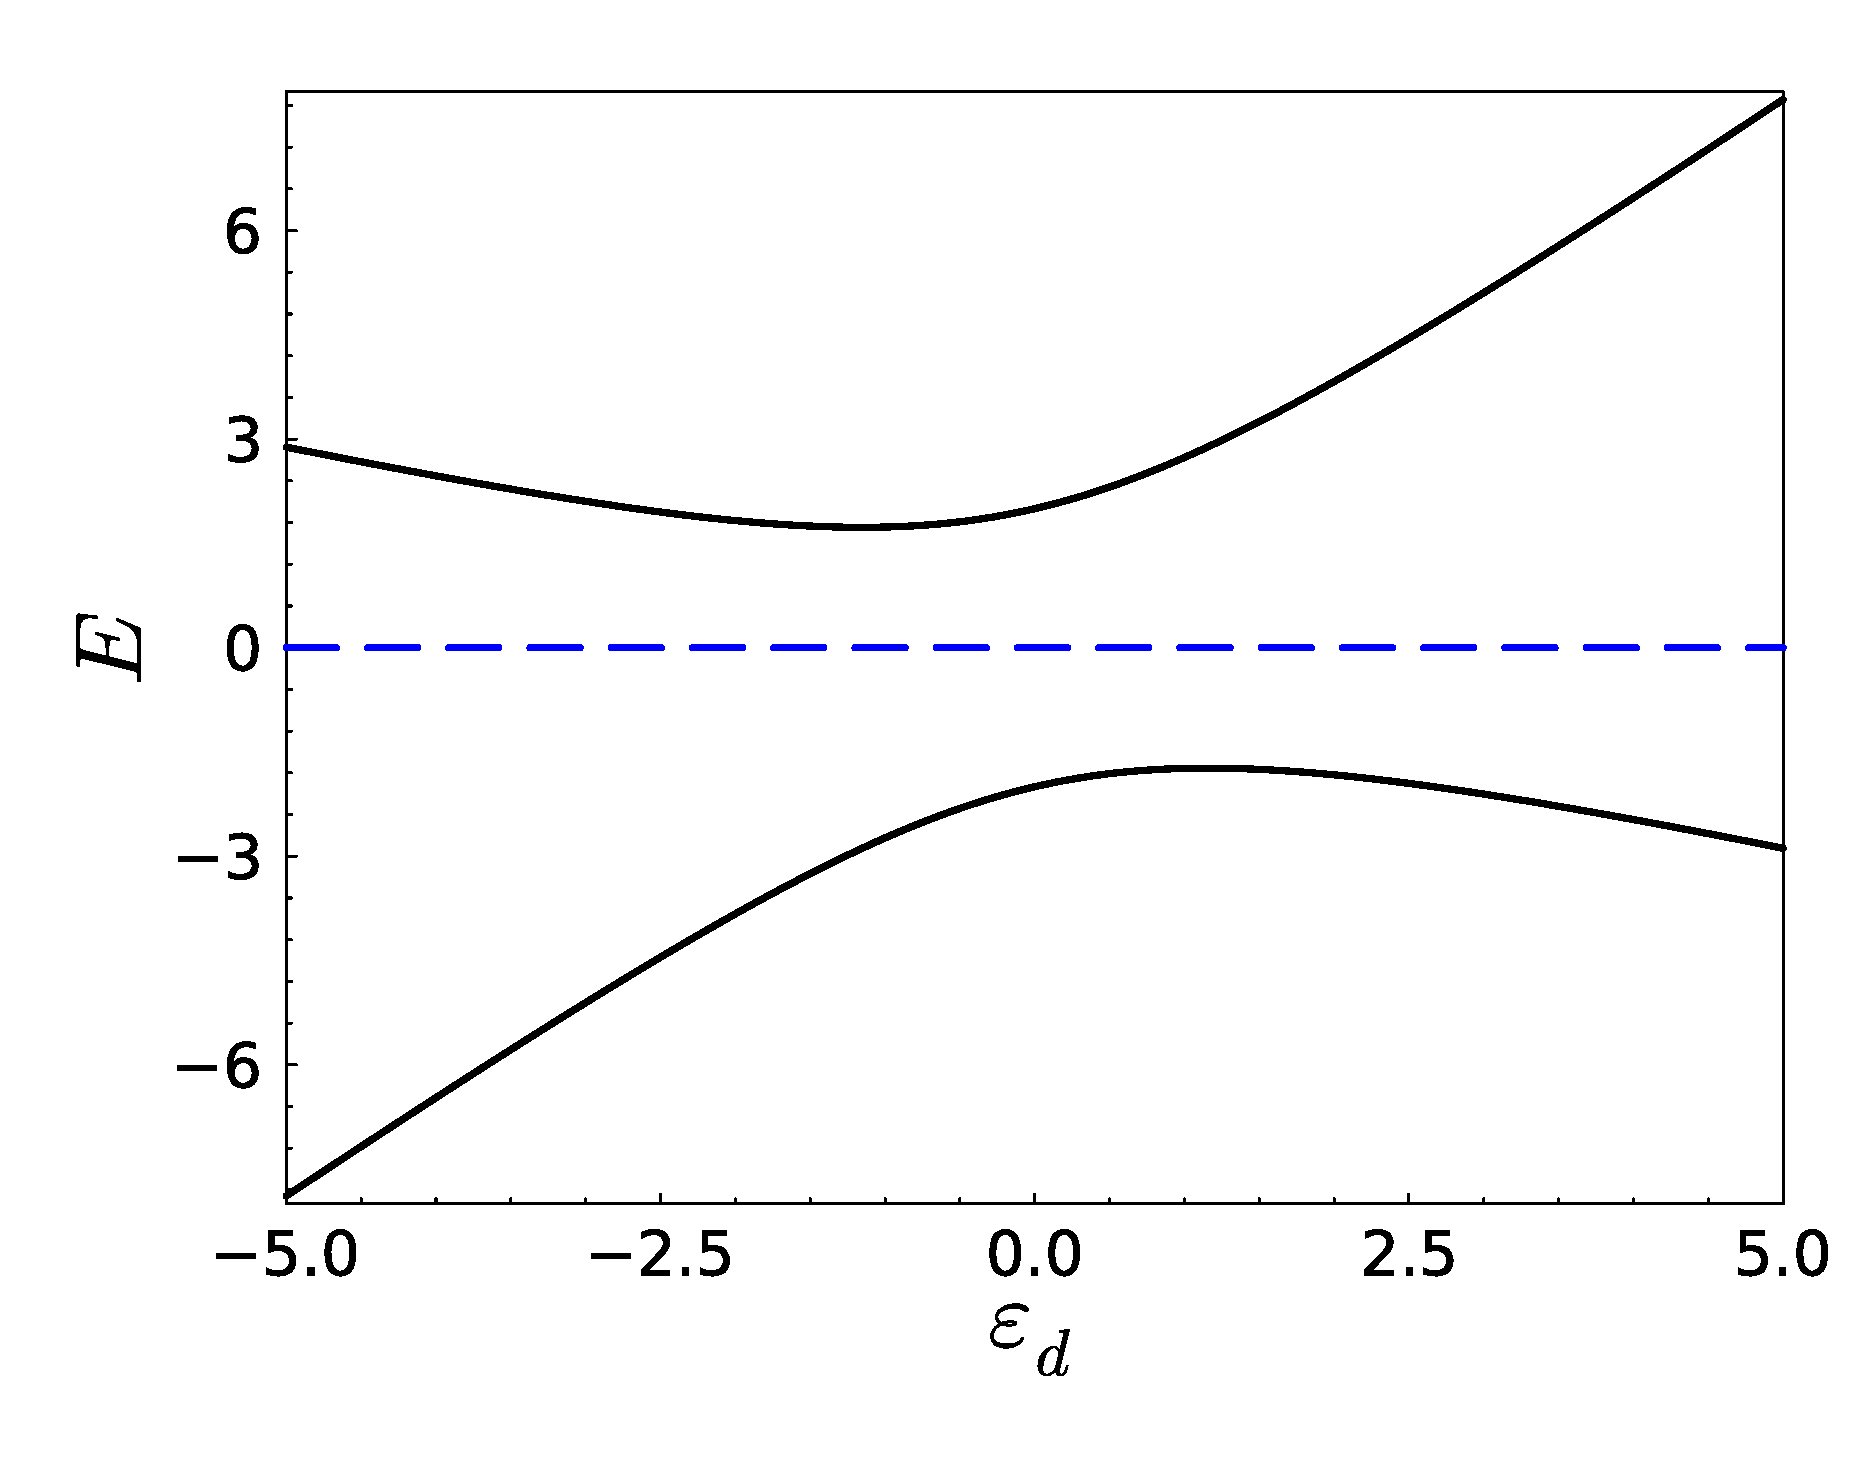
\includegraphics[width=0.70\textwidth]{molecula.pdf}
    \caption{Espectro de energ\'{i}as del modelo de la mol\'{e}cula diat\'{o}mica heteronuclear. Los par\'{a}metros del modelo fueron $t=1$ y $e_c=0$. El potencial qu\'{i}mico del primer sitio es mostrado por la l\'{i}nea punteada.}
    \label{fig:molecula}
\end{figure}
\end{comment}
%%%%%%%%%%%%%%%%%%%%%%%%%%%%%%%%%%%%%%%%%%%%%%%%%%%%%%%
%KITAEV
%
\begin{figure}[H]
\begin{center}
\includegraphics*[width=0.6\columnwidth]{ch3f/v0n20.pdf}\\
\vspace{-0.3cm}
\includegraphics*[width=0.6\columnwidth]{ch3f/v1n20.pdf}
\end{center}
\caption{Espectro de energ\'{i}as en funci\'{o}n de $\epsilon_d$ para una cadena de $N=20$ sitios con par\'{a}metros $\Delta=0.2$, $t=1$, $t'=0.2$ y $\mu=0$. La figura superior muestra el espectro de energ\'{i}as para cuando el t\'{e}rmino de repulsi\'{o}n es $V=0$, y la inferior para $V=1$.}
\label{comparacion1}
\end{figure} En las figuras \ref{comparacion2} para el caso de $N=50$ el nivel de robustez es mayor tal como se mencion\'{o} ya que vemos que para el caso de $N=20$ la separaci\'{o}n de los MZMs ten\'{i}a un tama\~{n}o de $\delta=0.02$ mientras que para esta cadena m\'{a}s grande es de $\delta=4.1\times 10^{-5}$.

Para una cadena de $N=50$, $t=1$ y $\Delta=t'=0.2$ analizamos de cerca el efecto que tiene la repulsi\'{o}n y el cambiar el potencial qu\'{i}mico de la cadena sobre los MZMs. La figura \ref{comparacion2}, donde el potencial qu\'{i}mico es $\mu=0$, curiosamente pasa lo opuesto a lo planteado por Ricco \emph{et alia}. Es decir, que cuando prendemos el t\'{e}rmino de repulsi\'{o}n, este en realidad mejora, aunque sea un poco, la calidad de los MZMs. Los vuelve m\'{a}s cercanos a una energ\'{i}a cero. Por otro lado, en la figura inferior de \ref{comparacion2}, se trata con el caso de un potencial qu\'{i}mico $\mu\neq 0$ que produce un perfil como el de un mo\~{n}o asim\'{e}trico consecuencia tanto de tener $\mu\neq 0$ y $V=1$. Si no se tienen ambos entonces el perfil sigue siendo el del mo\~{n}o sim\'{e}trico.
%
% upclose V=0 vs V=1 en una sola grafica
% 
\begin{figure}[H]
\begin{center}
\includegraphics*[width=0.7\columnwidth]{ch3f/compa0.pdf}\\
\vspace{-0.3cm}
\includegraphics*[width=0.7\columnwidth]{ch3f/compa05.pdf}
\end{center}
\caption{Comparaci\'{o}n de las dos energ\'{i}as m\'{a}s cercanas a cero como funci\'{o}n de $\epsilon_d$ entre $V=0$ y $V=1$ para distintos valores del potencial qu\'{i}mico $\mu$ ($\mu=0$ imagen superior y $\mu=0.5$ imagen inferior) para una cadena de $N=50$ sitios con par\'{a}metros de $\Delta=0.2$, $t=1$ y $t'=0.2$.}
\label{comparacion2}
\end{figure}

Como hab\'{i}amos mencionado en el argumento, una vez el hamiltoniano es diagonalizado, los nuevos operadores que diagonalizan el Hamiltoniano son en realidad una combinaci\'{o}n lineal de los operadores fermionicos usados para escribir el $H$ original. El autoestado de m\'{a}s baja energ\'{i}a con energ\'{i}a positiva (as\'{i} como todos los dem\'{a}s) tiene la forma 
\begin{equation}
    \gamma_\nu^\dagger=\sum_{i}\Big( \overline{A}_{i\nu}c_{i}+\overline{B}_{i\nu'}c^\dagger_{i} \Big). 
\end{equation}
donde $E_\nu\approx 0$. M\'{a}s explicitamente, para el operador de aniquilaci\'{o}n:
\begin{equation}
    \begin{split}
        \gamma_\nu &= A_{0\nu} d^\dagger + B_{0\nu} d\\
     &+ A_{1\nu} c_1^\dagger + B_{1\nu} c_1\\
     &+ ...\\
     &+ A_{50\nu} c_{50}^\dagger + D_{50\nu} c_{50}
    \end{split} 
\end{equation}
Este autoestado, como se espera seg\'{u}n la propuesta original de Kitaev, y a diferencia de los otros autoestados, deber\'{i}a tener entre sus coeficientes de mayor peso a los coeficientes que acompa\~{n}an a los operadores de los extremos de la cadena que es precisamente lo que se ve en \ref{fig: wm1}. La peculiaridad aqu\'{i} es que a diferencia de la cadena de Kitaev, hay un peso relevante en el punto cu\'{a}ntico. 
%
% Operator index vs position in chain
%
\begin{figure}[H]
    \centering
    \includegraphics[width=0.70\textwidth]{ch3f/wm1.pdf}
    \caption{Coeficientes del estado de m\'{a}s baja energ\'{i}a. Los par\'{a}metros de la cadena son $N=50$, $t=V$, $\Delta=t'=0.2$, $\epsilon_d=-1$ y $\mu=0$.}
    \label{fig: wm1}
\end{figure}
En la secci\'{o}n 1.3 se habl\'{o} del modelo de Prada \emph{et alia}. Los autores encontraron que para un cable largo ($L=2$ $\mu$m) el espectro a bajas energ\'{i}as los MZMs est\'{a}n topol\'{o}gicamente protegidos, mientras que para un cable corto ($L=400$ nm) los MZMs formaban patrones de mo\~{n}o o diamante. Por lo tanto suena razonable el querer aplicar lo mismo en nuestro modelo y encontrar los mismos patrones que Prada \emph{et alia} encontraron para el caso de la cadena corta. Con una relaci\'{o}n de $\frac{1}{10}$, nosotros ahora pasamos de cadenas de un tama\~{n}o de $N=50$ sitios, a ver sistemas de $N=5$. Las im\'{a}genes de la figura \ref{cortito} muestran que para una cadena de $N=5$ sitios obtenemos el mismo patr\'{o}n de diamante que ellos. 

Con los resultados anteriores sab\'{i}amos que al aumentarle la cantidad de sitios los MZMs solo se hac\'{i}an m\'{a}s robustos porque cuanto m\'{a}s largo es el cable menos importa el efecto de repulsi\'{o}n. Por lo tanto, solo quedaba ver qu\'{e} era lo que pasaba cuando ten\'{i}amos cables muy cortos.
Entonces, para el caso de cables cortos, el efecto de repulsi\'{o}n s\'{i} es relevante ya que si bien hay una separaci\'{o}n de energ\'{i}as ya existente en la figura \ref{cortito} para un $V=0$, para $V=1$ se ve que la separaci\'{o}n de energ\'{i}as es much\'{i}simo mayor al punto que podemos decir que estos ya no son MZMs, pues se encuentran muy alejados de una energ\'{i}a cero. La explicaci\'{o}n para esto es que el cable cu\'{a}ntico al ser muy peque\~{n}o, favorece hibridaci\'{o}n o mezcla de los Majoranas de energ\'{i}a cero, y, por consecuencia, la protecci\'{o}n que ellos usualmente adquieren al estar cerca a cero se ve comprometida.
%%%%%%%%%%%%%%%%%%%%%%%%%%%%%%%%%%%%%%%%%%%%%%%%%%%%%%%
%KITAEV
%
\begin{figure}[H]
\begin{center}
\includegraphics*[width=0.5\columnwidth]{ch3f/diaV0.pdf}\\
\vspace{-0.3cm}
\includegraphics*[width=0.5\columnwidth]{ch3f/diaV1.pdf}
\end{center}
\caption{Espectro a bajas energ\'{i}as como funci\'{o}n de $\epsilon_d$ para los casos $V=0$ y $V=1$. Los par\'{a}metros de la cadena son $N=5$, $t=1$, $\Delta=t'=0.2$ y $\mu=0$. }
\label{cortito}
\end{figure}%%%%%%%%%%%%%%%%%%%%%%%%%%%%%%%%%%%%%%%%
